% Template:     Informe LaTeX
% Documento:    Archivo de ejemplo
% Versión:      8.1.7 (24/07/2022)
% Codificación: UTF-8
%
% Autor: Pablo Pizarro R.
%        pablo@ppizarror.com
%
% Manual template: [https://latex.ppizarror.com/informe]
% Licencia MIT:    [https://opensource.org/licenses/MIT]

\section{Introducción}

Amazon.com, Inc. Amazon, una empresa estadounidense de comercio electrónico y computación en la nube, fue fundada en julio de 1994. Es conocida por la tienda más grande del mundo de CD, libros, piezas de repuesto para automóviles, juguetes para niños, productos electrónicos, hardware, etc. También es conocida por fabricar artículos de consumo. electrónica: Amazon Kindle, Amazon Alexa, Echo y muchos más. Amazon también permitió que los autores y editores publicaran y pusieran a disposición sus libros en Kindle Store, con el brazo de publicación "Amazon Publishing". \scite{jopson2011amazon}

\begin{figure}[h]
	\centering
	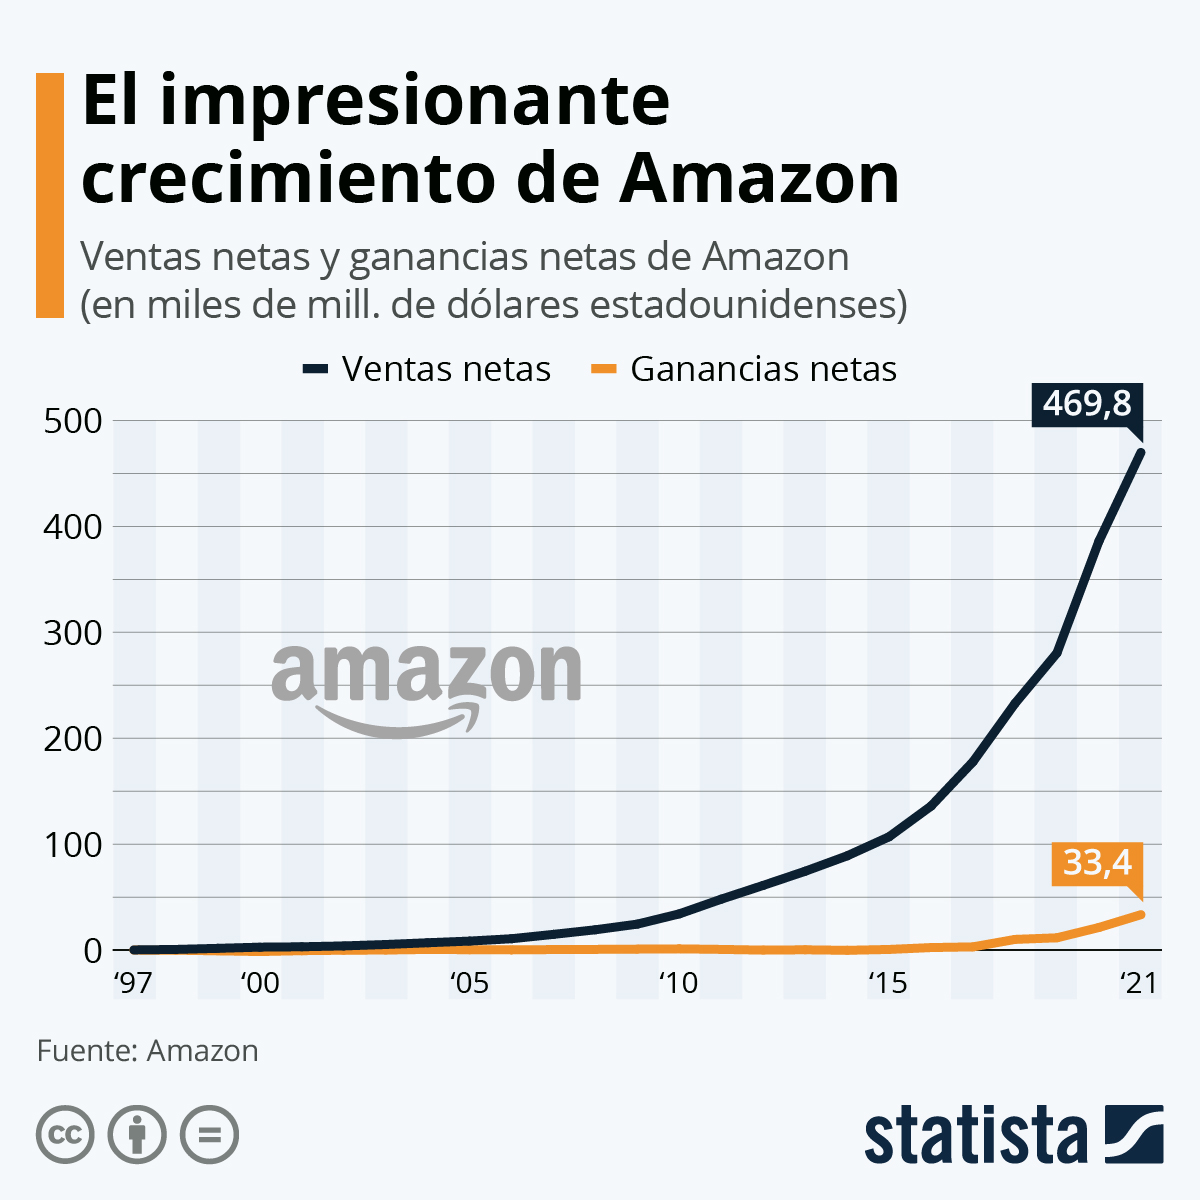
\includegraphics[scale=.2] {img/crecimiento_amazon}
	\caption{Crecimiento}
	\label{fig:1}	
\end{figure}

Amazon es el quinto sitio web más visitado a nivel mundial, con un total de 3,000 millones de visitas a septiembre de 2021, según datos de Semrush. El portal de comercio electrónico también registró 0.7 mil millones de visitantes únicos. \scite{semrush}

\subsection{Procesamiento y almacenamiento}
El sistema se evalúa en el catálogo de productos de Amazon, un gran conjunto de datos que comprende alrededor de 9 millones de productos, 144 millones de reseñas y una gran cantidad de metadatos \scite{singh2019analysis}

\subsection{¿Cuál es su necesidad?}

El sistema se evalúa en el catálogo de productos de Amazon, un gran conjunto de datos que comprende alrededor de 9 millones de productos, 144 millones de reseñas y una gran cantidad de metadatos \scite{singh2019analysis}

\subsection{Amazon EMR Architecture \& Working}
Amazon mezcla y combina arquitecturas para satisfacer sus diversas necesidades comerciales. Amazon EMR Model analiza el mapa y reduce el big data. Amazon Elastic MapReduce proporciona usos sistemáticos y sencillos de la plataforma de análisis dentro del poderoso marco Hadoop que utilizan en gran medida algunas grandes empresas. El funcionamiento de Amazon EMR se basa en la arquitectura maestro/esclavo, mientras que el trabajo de Amazon EMR se basa en la arquitectura maestro/esclavo, mientras que los nodos maestros son parte del grupo de instancias de MapReduce y los nodos esclavos aún ejecutan HDFS y se convierten en más nodos principales. Las arquitecturas se ejecutan en la siguiente secuencia:
\begin{itemize}
	\item Amazon EMR envía una solicitud para iniciar un clúster.
	\item Amazon EMR crea el clúster de Hadoop con un nodo principal agregado a la instancia principal y un nodo central agregado al grupo principal.
	\item Un solo nodo maestro y muchos otros nodos esclavos procesan las tareas en el clúster.
\end{itemize}



“Amazon utiliza Amazon Elastic MapReduce (Amazon EMR) para sus procesos comerciales de comercio electrónico y en el análisis de una gran cantidad de datos distribuidos, administrados por el marco Hadoop, es rápido y rentable, adecuado para compras bajo demanda. Amazon EMR funciona en varios clústeres y los servidores se ejecutan en la arquitectura de nube distribuida de Amazon y administra big data, incluidos archivos de registro, indexación web, simulación científica, extracción de datos, almacenamiento de datos, inteligencia artificial y análisis de contabilidad seguros y confiables” \scite{zakir2015big}

\begin{figure}[h]
	\centering
	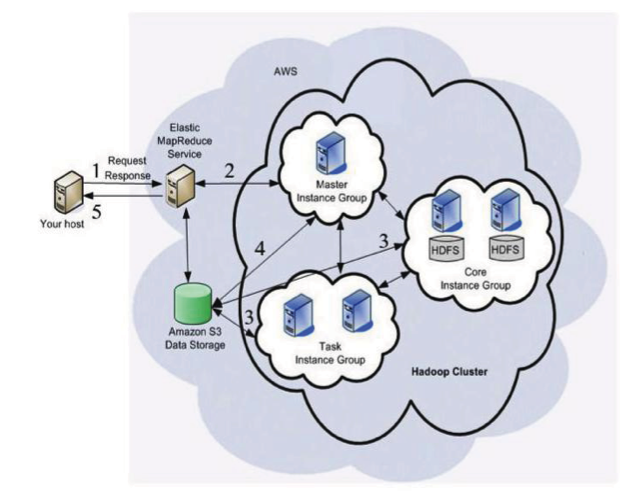
\includegraphics[scale=.4] {img/A-EMR-Arch}
	\caption{Amazon EMR Architecture}
	\label{fig:2}	
\end{figure}

AMAZON HADOOP: Hadoop es un concepto de marco de código abierto que admite la técnica de procesamiento de datos en un controlador de clúster múltiple de Amazon que utiliza una arquitectura maestra y esclava en muchos servidores. Amazon utiliza Amazon MapReduce para el procesamiento de grandes datos y para el almacenamiento de datos utiliza HDFS \scite{zakir2015big}
\begin{figure}[h]
	\centering
	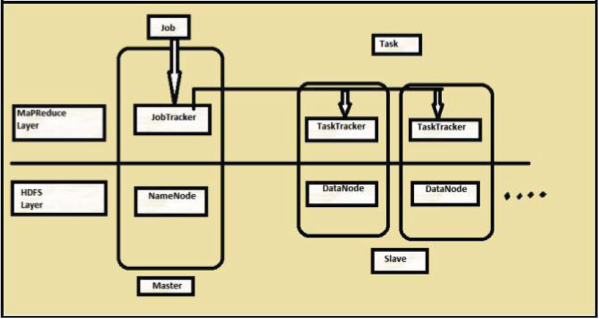
\includegraphics[scale=.4] {img/hadoop-w}
	\caption{Hadoop working, Fuente: \scite{verma2018beyond}}
	\label{fig:3}	
\end{figure}


Amazon desarrolló sofisticados motores de recomendación que entregan más del 35\% de todas las ventas soportadas en Big Data, sistemas automatizados de servicio al cliente para garantizar una satisfacción superior del cliente y sistemas de precios dinámicos que ajustan los precios en comparación con los sitios de la competencia \scite{agarwal2014big}

\subsection{El proceso de Big Data de Amazon}

El proceso de big data \scite{chen2017application} de Amazon se divide en tres etapas: recopilación y aplicación artificial, sistema de recomendación principal, que fue más complejo para construir el sistema de datos, como la Figura \ref{fig:4}. y sistema de información logística, nuevo sistema de recomendación de datos y sistema de gestión logística, como Figura \ref{fig:5}. 

\begin{figure}[h]
	\centering
	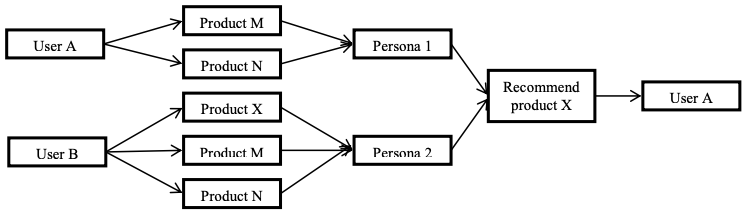
\includegraphics[scale=.5] {img/recomendation-system}
	\caption{Sistema de recomendación por asociación de usuario: \scite{singh2019analysis}}
	\label{fig:4}	
\end{figure}

\begin{figure}[h]
	\centering
	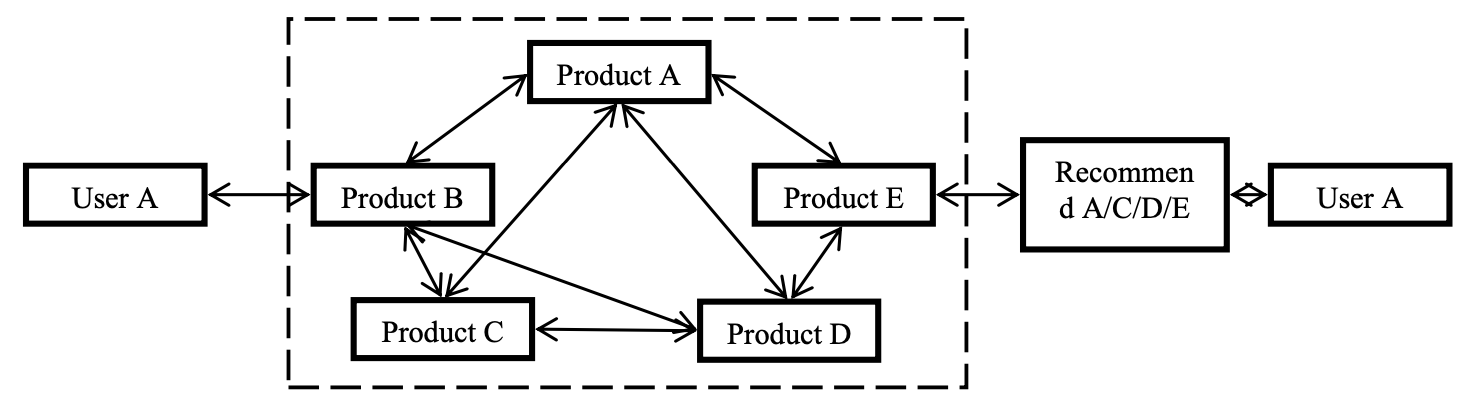
\includegraphics[scale=.3] {img/asocacion_productos}
	\caption{Sistema de recomendación por asociación de productos, Fuente: \scite{singh2019analysis}}
	\label{fig:5}	
\end{figure}



% ------------------------------------------------------------------------------
% NUEVA SECCIÓN
% ------------------------------------------------------------------------------
% Las secciones se inician con \section, si se quiere una sección sin número se
% pueden usar las funciones \sectionanum (sección sin número) o la función
% \sectionanumnoi para crear el mismo título sin numerar y sin aparecer en el índice
\section{Cuál es su necesidad}

\lipsum[2] % Párrafo ejemplo, se puede borrar	


% ------------------------------------------------------------------------------
% NUEVA SECCIÓN
% ------------------------------------------------------------------------------
\clearpage
\section{Cómo lo utiliza}

\lipsum[2] % Párrafo ejemplo, se puede borrar	

% ------------------------------------------------------------------------------
% NUEVA SECCIÓN
% ------------------------------------------------------------------------------
% Inserta una sección sin número
\clearpage
\section{Las 4`V de Big Data de Amazon }
\subsection{Volumen}

\lipsum[1] % Párrafo ejemplo, se puede borrar	

\subsubsection{Cuál es el volumen de datos que almacena}
\lipsum[1] % Párrafo ejemplo, se puede borrar	

\subsubsection{Cuál es el volumen de datos que procesa}
\lipsum[1] % Párrafo ejemplo, se puede borrar	

% ------------------------------------------------------------------------------
% NUEVA SECCIÓN
% ------------------------------------------------------------------------------
\clearpage

\subsection{Variedad}
Las empresas Amazon, capturan varios tipos de datos (p. ej., pedidos, carrito de compras, visitas, usuarios, enlaces de referencia, palabras clave, búsqueda de catálogos, datos sociales), que pueden clasificarse en términos generales en cuatro categorías: (a ) datos de transacciones o actividades comerciales (b) datos de flujo de clics (c) datos de video y (d) datos de voz (ver Tabla 5). En el comercio electrónico, los datos son la clave para rastrear el comportamiento de compra del consumidor para personalizar las ofertas, que se recopilan a lo largo del tiempo mediante la navegación del consumidor y los puntos transaccionales. Analizamos  diferentes tipos de macrodatos junto con sus implicaciones para el comercio electrónico de Amazon.


\begin{table}[h]
\resizebox{\textwidth}{!}{%
\begin{tabular}{lll}
\hline
\multicolumn{1}{c}{\textbf{Tipo}} &
  \multicolumn{1}{c}{\textbf{Descripción}} &
  \multicolumn{1}{c}{\textbf{Aplicaciones para e-bussiness}} \\ \hline
\begin{tabular}[c]{@{}l@{}}Datos de transacciones o \\ actividades comerciales\end{tabular} &
  \begin{tabular}[c]{@{}l@{}}Datos estructurados de transacciones minoristas, \\ perfiles de clientes, frecuencia y volumen de \\ distribución, consumo de productos y uso de \\ servicios, naturaleza y frecuencia delas quejas \\ de los clientes\end{tabular} &
  \begin{tabular}[c]{@{}l@{}}Amazon utiliza un tipo de técnica de modelado predictivo \\ 
                             llamada filtrado colaborativo, que utiliza los datos de \\ 
                             los clientes para generar avisos de "es posible que también\\ 
                             desee" para cada producto comprado o visitado. Amazon \\ 
                             reveló en un momento que el 30\% de las ventas se generaron\\
                             a través de su motor de recomendaciones \scite{manyika2011big}.\end{tabular} \\
Click-stream data &
  Datos de flujo de clics de la web, anuncios en línea &
  \begin{tabular}[c]{@{}l@{}}El estudio actual simula el tráfico mensual de Amazon en \\ EE. UU., que se estima en 175 millones de visitas únicas por \\ mes en una base de datos de 300 millones de productos.\end{tabular} \\
Datos de Audio y Video &
  Datos de vide y otras configuraciones &
  \begin{tabular}[c]{@{}l@{}}En el sitio web: \href{https://www.amazon.es/gp/help/customer/display.html?nodeId=GXPU3YPMBZQRWZK2}{'Solicitar mis datos'}  podemos solicitar los \\ datos almacenados por nosotros  como usuarios de \\ diversos servicios, entre ellos, AmazonMusic, \\ PrimeVideo, entre otros \scite{amazon-data} \end{tabular} \\ \hline
\end{tabular}%
}
\end{table}


La variedad son los datos que se recopilan de diferentes fuentes en lugar de formas no estructuradas, estructuradas o semiestructuradas. Amazon hace uso del concepto de big data. Son más de 2.000 datos históricos y en tiempo real. Hace uso de algoritmos de aprendizaje automático en cada uno de sus pedidos realizados por el usuario. Recopila una variedad de datos a través de:

\begin{itemize}
	\item Rastreadores de actividad física, 
	\item cámaras como amazon echo show, 
	\item Sistemas de música como Amazon Music, 
	\item Lectores audibles como kindle, 
	\item video streaming como Amazon prime video, etc.
\end{itemize}

Además de la información que nos proporcionas, recopilamos información automáticamente cuando interactúas con nuestro sitio web o nuestros productos y servicios, para mejorar tu experiencia con Amazon.
Las formas más comunes en las que nos proporcionas información incluyen búsquedas de productos o servicios, la realización de pedidos o cuando te pones en contacto con nosotros para solicitarnos ayuda. Algunos ejemplos de la información que nos proporcionas son tus datos de contacto y de entrega, información de pago u otras preferencias \scite{amazon}


% ------------------------------------------------------------------------------
% NUEVA SECCIӓN
% ------------------------------------------------------------------------------
\clearpage
\subsection{Velocidad}

\subsubsection{Cuanto es el tiempo en que procesaba antes de usar Hadoop}
\lipsum[1]\scite{verma2018beyond} % Párrafo ejemplo, se puede borrar	

\subsubsection{Cuanto es el tiempo que procesa ahora que usa Hadoop}


% ------------------------------------------------------------------------------
% NUEVA SECCIӓN
% ------------------------------------------------------------------------------
\clearpage
\subsection{Veracidad}

\subsection{Como probar que los datos que procesa sean válidos}
\lipsum[1] % Párrafo ejemplo, se puede borrar	

% ------------------------------------------------------------------------------
% REFERENCIAS, revisar configuración \stylecitereferences
% ------------------------------------------------------------------------------
\clearpage
\bibliography{library}